\section{Einleitung}
Mit der zunehmenden Globalisierung steht heute praktisch jedes produzierende Unternehmen 
im internationalen Wettbewerb. Der Markt fordert hohe Flexibilität und Lieferfähigkeit, 
wobei die Kosten immer weiter sinken sollen, um wettbewerbsfähig zu bleiben.
Die japanische Firma Toyota hat diese Problematik für sich bereits in den 1950er
Jahren erkannt und eigene Lösungen dafür gesucht. So ist schliesslich im Laufe der
folgendenden Jahrzehnte das \emph{Toyota-Produktionssystem} (TPS) entwickelt worden, dessen 
wesentliche Bestandteile heute auch unter den Begriffen  \emph{Just-in-Time} oder  
 \emph{Lean-Production} bekannt sind. Ein wichtiger Bestandteil des TPS ist das
Kanban-System, das vor allem von Taiichi Ohno entwickelt wurde.
\footnote{vgl. \cite{Ohno2013TPS} S.39}\\
Die vorliegende Arbeit gibt eine Einführung in die wesentlichen Methoden, 
Werkzeuge und Prinzipien des Kanban-Systems und wie mit Hilfe von Kanban eine
Just-in-Time-Produktion umgesetzt werden kann. Im zweiten Abschnitt wird hierzu
die Geschichte und Entwicklung von Kanban vorgestellt.
Im Abschnitt drei wird aufgezeigt, wie Kanban im produzierenden Betrieb 
eingeführt werden kann und wie dadurch die Wettbewerbsfähigkeit gesteigert wird. 
Eng in Verbindung mit Kanban steht der kontinuierliche Verbesserungsprozess 
(KVP), auch Kaizen genannt, was im vierten Abschnitt betrachtet wird.
Im letzten Abschnitt wird kritisch auf die Risiken einer Kanban-Einführung
eingegangen und ein Ausblick auf die zu erwartende künftige Entwicklung gegeben.\\
Für die Erstellung dieser Arbeit wurde auf relevante Fachliteratur zurückgegriffen
und teilweise auch im Internet recherchiert.

\section{Geschichte und Entwicklung von Kanban}

Das Toyota-Produktionssystem entand im Japan der Nachkriegszeit 
aus der wirtschaftlichen Notwendigkeit heraus. 
Die Produktivität eines japanischen Arbeiters betrug zu der Zeit nur einen Bruchteil der Produktivität eines Amerikaners. 
Der damalige Präsident der Toyota Motor Company Kiichiro Toyoda (1894-1952) gab daher das Ziel vor, 
die US-amerikanische Automobilindustrie innerhalb von drei Jahren  einzuholen. \footnote{vgl. \cite{Ohno2013TPS} S.36}\\
Toyotas Produktionsleiter Taiichi Ohno war der Ansicht, man müsse alle Arten von 
Verschwendung von Material und Zeit und alle unproduktiven Tätigkeiten 
beseitigen, um den Rückstand aufzuholen. Als eine Hauptursache der Ineffizienz 
und Verschwendung identifizierte man bei Toyota die Überproduktion bzw. die Produktion auf 
Halde und damit verbunden übermässige Lagerhaltung. Dadurch wird Kapital gebunden, 
die Duchlaufzeiten erhöhen sich, durch Korrosion und häufigen Transport verschlechtert
sich die Qualität der Zwischenerzeugnisse und möglicherweise müssen soger zu viel
produzierte Teile weggeworfen werden. Bedingt durch die räumliche Enge stellt die 
Lagerhaltung in Japan auch prinzipiell ein höheren Kostenfaktor dar als beispielsweise in den USA.
Künftig sollte bei Toyota die Fließproduktion \emph{Just-in-Time} erfolgen. 
Das bedeutet, dass die für die Produktion benötigten Teile zur rechten Zeit und 
nur in der benötigten Menge am Fließband ankommen.
Toyota kam dabei zu Gute, dass das Werk in einer Region mit vielen Zulieferer-Firmen (ein sog. Cluster der Autoindustrie)
lag und die Anlieferung von Teilen daher schnell und kurzfristig möglich war. \footnote{vgl. \cite{Economist2009Ohno} S.36}
Auf diese Weise sollte der Lagerbestand auf ein Minimum reduziert werden.
Mit den herkömmlichen Verfahren zur Produktionsplanung vom Rohstoff 
bis zum Endprodukt war das nicht zu schaffen.
Stattdessen betrachtete Ohno den Materialfluss vom Ende her, also in entgegengesetzter Richtung.
Eine Produktionsstufe entnimmt sich die benötigten Teile von der vorgelagerten Stufe oder dem Zwischenlager,
die vorgelagerte Stufe produziert darauf hin die entnommene Menge an Teilen nach.
So entsteht ein sich selbst regelndes System von Produzent und Verbraucher.
Ohno verglich das System gerne mit einem Supermarkt, wo ganz ähnlich die Regale wieder aufgefüllt werden, 
sobald die Kunden eine gewisse Menge an Waren entnommenhaben. 
Ohno nennt dieses selbststeuernde System daher auch das \emph{Supermarktsystem}.\footnote{vgl. \cite{Ohno2013TPS} S.61}

Für die Informationsübertragung in diesem Regelkreis dienen die Kanban-Karten.
Das Wort \emph{Kanban} besteht aus den zwei Zeichen {\CN 看} ( \emph{kan}=sehen)
 und {\CN 板} (\emph{ban}=Tafel, Brett) und läßt sich etwa mit Sichttafel, 
 Aushängeschild oder auch Pendelkarte übersetzen.

Im Produktionsprozess steht jede Kanban-Karte für einen Behälter einer bestimmten Größe, der eine festgelegt Anzahl von Bauteilen enthält.
Die Kanban-Karte wird an dem entsprechenden gefüllten Behälter befestigt oder eingesammelt und wieder zurück zum 
Produzenten der Teile gebracht, als Information dafür, dass wieder neue Teile benötigt werden. 
Dafür muss die Kanban-Karte verschiedene Informationen enthalten, wie Bezeichnung und Nummer der Teile, 
Anzahl der Teile pro Behälter, Art des Behälters, Produzent und Verbraucher der Teile und ggf. auch Strichcodes für die elektonische Datenerfassung.
(s. Abbildung \ref{Kanbankarte})
\begin{figure}[h]
\centering
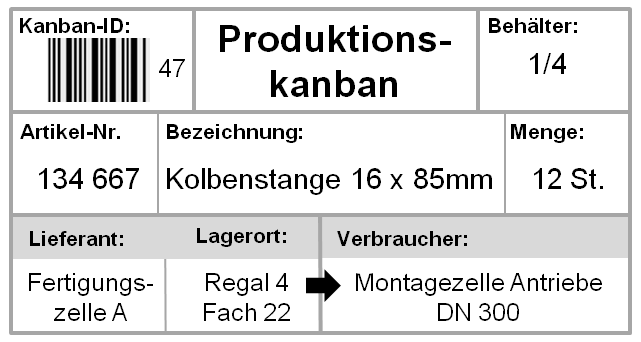
\includegraphics[width=.60\textwidth]{img/kanban-karte.png}
\caption[Beispiel einer Kanban-Karte]{Beispiel einer Kanban-Karte\footnotemark}
\label{Kanbankarte}
\end{figure}
\footnotetext{Quelle: http://www.lean-production-expert.de/lean-production/kanban-kartengestaltung.html}

Die Anzahl von Kanban-Karten für ein Bauteil oder eine Bauteilgruppe ist begrenzt, auf diese Weise soll verhindert werden, dass zu viel auf Lager produziert wird.
Der gesamte Produktionsprozess wird nun betrachtet als eine Aneinanderreihung von Quellen und Senken von Produktionsgütern, mit kleinen Zwischenlagern als Puffer.
Eine Senke nimmt sich einen Behälter aus dem Zwischenlager (Pull-Prinzip), verarbeitet alle Teile darin und füllt selbst als Quelle das nachgelagerte Zwischenlager.
(s. Abbildung \ref{flow})
\begin{figure}[h]
\centering
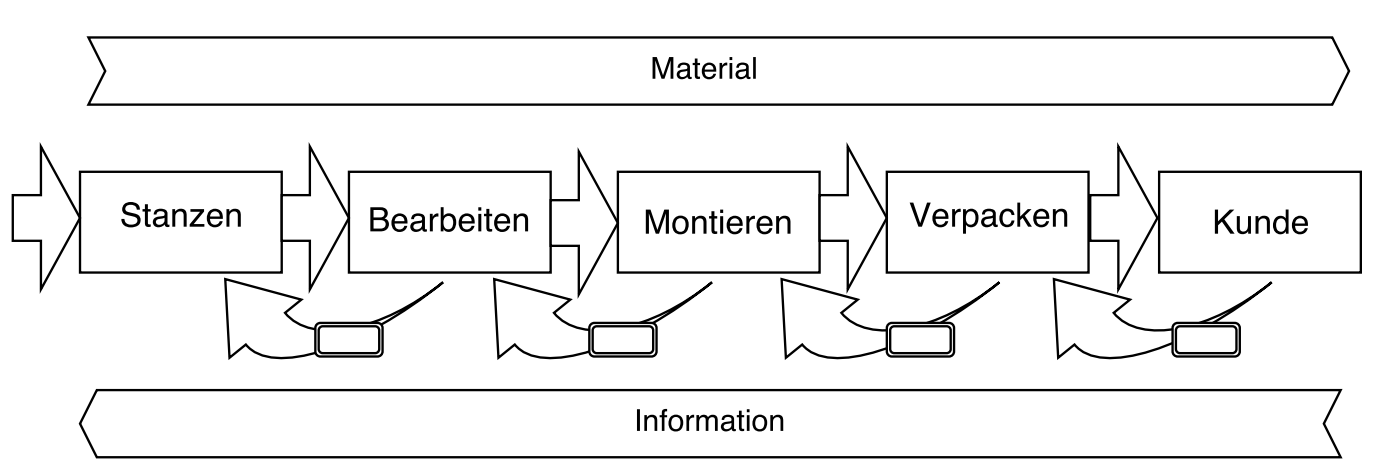
\includegraphics[width=.90\textwidth]{img/kanban-flow.png}
\caption[Regelkreise mit Fluß von Informationen und Material]{Regelkreise mit Fluß von Informationen und Material\footnotemark}
\label{flow}
\end{figure}
\footnotetext{eigene Darstellung}

Hat das nachfolgende Zwischenlager einen bestimmten Höchststand überschritten, \emph{darf nicht} weiter produziert werden.
Wird dagegen ein bestimmter Mindeststand unterschritten, so \emph{muss} wieder Nachschub produziert werden.
Auf diese Weise werden Probleme oder Engpässe schnell sichtbar und es können entsprechende Gegenmaßnahmen unternommen werden.
Andererseits können durch die mehrstufigen Zwischenlager Schwankungen bei Nachfrage, Zulieferung oder Personalstärke in gewissen Grenzen ausgeglichen werden.

Die Zwischenlager der einzelnen Produktionsstufen können auf einer \emph{Plantafel} (auch Kanban-Tafel) visualisiert werden, welche an zentraler Stelle für alle Beteiligten gut sichtbar platziert wird.
Für jede Produktionsstufe gibt es auf der Plantafel eine Spalte oder Zeile mit festen Plätzen für die Kanban-Karten.
Die Karten der leeren Behälter werden hier für jeden sichtbar plaziert, so dass auf einen Blick der Bestand der Zwischenlager erkennbar wird.

\section{Einführung von Kanban}
\subsection{Problemstellung}
Die Motivation für die Einführung der Just-in-Time-Produktion ist heute die gleiche wie im 20. Jahrhundert bei Toyota.
Bei gleichbleibend hoher Qualität sollen Lieferfähigkeit und Flexibilität gesteigert werden.
Ebenso sollen Durchlaufzeiten und Umlaufvermögen reduziert werden.\footnote{vgl. \cite{Geiger2011Kanban} S.12}
Hinzu kommt heute noch, dass herkömmliche PPS-Systeme einen hohen Aufwand bedeuten, 
sowohl bei der Produktionsplanung als auch bei der Erfassung von Daten zu Lagerbeständen und produzierten Gütern.
Dabei sind die eingesetzten IT-Systeme oft zu unflexibel und zu theoretisch.\footnote{vgl. \cite{Weber2014KE} S.1}\\
Trotz Einsatz moderner Technik kommt es zu Unstimmigkeiten von tatsächlichem und theoretischem Bestand, 
was eine Störung der Produktion zur Folge haben kann.
Diese nicht wertschöpfenden Tätigkeiten können durch die Einrichtung der selbstregelnden 
Steuerkreise eines Kanban-Systems eliminiert oder zumindest stark reduziert werden.\footnote{vgl. \cite{Geiger2011Kanban} S.13}

\subsection{Vorgehensweise}
Die Einführung der JIT-Fertigung nach dem Kanban-System sollte immer schrittweise erfolgen,
so hat man die Möglichkeit, zuerst in einem kleinen Teilbereich Erfahrung zu 
sammeln und eventuell bereite erste Verbesserungen vorzunehmen. 
Dabei fängt man gemäß dem Pull-Prinzip am Ende der Wertschöpfungskette an, 
also dem Fertigteilelager oder der Endfertigung. 
In diesem Teilbereich organisiert sich ein Team von ca. 10 Personen eigenständig, zunächst für eine Dauer von 6-12 Monaten.\\
Schrittweise wird das Kanban-System dann auf die vorgelagerten Produktionstufen ausgeweitet, 
um zuletzt auch den Einkauf und die Lieferanten einzubeziehen.\footnote{vgl. \cite{Takeda2012SPS} S.194}
Von allen Beteiligten müssen die Kanban-Regeln verstanden sein und eingehalten werden. 
Dazu müssen sie entsprechend geschult werden und können mit Planspielen auf die Umstellungen vorbereitet werden.
Günstig ist es, die Regeln in einfacher Form für jeden sichtbar darzustellen und hier auch den 
Kanban-Beauftragten als Ansprechpartner bei Fragen und Problemen zu benennen.

\subsection{Kanban-Regeln}
Die Regeln für die JIT-Fertigung mit Kanban müssen allen Beteiligten kommuniziert und klar gemacht werden.
Für die Mitarbeiter in den Fertigungs-Teams können beispielsweise folgende Regeln vereinbart werden: \footnote{\cite{Weber2014KE} S.99}\\
\begin{enumerate}
\item Teile werden nur in festen Mengen bzw. Standardbehältern gelagert oder transportiert.
\item Jedem Kanban-Behälter ist eine Kanban-Karte zugeordnet.
\item Ist ein Kanban-Behälter geleert, so ist die Nachlieferung mit Hilfe der zugeordneten Kanban-Karte umgehend bei den betreffenden Lieferanten anzustoßen.
\item Jede Kanban-Karte auf der Steuer-/Auslastungstafel gilt als Auftrag in der vorgegebenen Menge zum vorgegebenen Termin. Ohne Kanban-Karte keine Fertigung, kein Arbeitsprozess, kein Transport.
\item Die Anzahl der Kanban-Karten darf nicht eigenmächtig verändert werden, es dürfen auch keine Änderungen der Daten auf der Kanban-Karte vorgenommen werden. Für die Pflege der Karten wird ein Karten-Pate bestimmt.
\item Nur vollständige Kanban-Behälter mit fehlerfreien Teilen dürfen weitergegeben werden. Zu jedem Behälter gehört eine Kanban-Karte. Teile dürfen nur in den vorgeschriebenen Behältern aufbewahrt und geliefert werden. Nullfehler-Organisation / Mitarbeiter-Selbstkontrolle
\item Kanban-Behälter dürfen nur an den zugewiesenen Plätzen abgestellt werden (Festplatzsystem). Kanban-Termine müssen zu 100\% eingehalten werden. Kanban-Aufträge haben immer höchste Priorität (Intercity-System).
\item Die Kanban-Auslastungstafeln müssen einwandfrei geführt werden, bei Engpässen Meldung an Vorgesetzte.
\item Den jeweiligen Fertigungsbeginn bestimmen die Mitarbeiter selbst gemäß festgelegter Lieferzeit auf der Kanban-Karte. Früher darf geliefert werden, später nie.
\end{enumerate}
Die einzelnen Details der Regeln sind natürlich den Gegebenheiten vor Ort anzupassen.
Generell ist das Kanban-System flexibel und macht keine strikten Vorgaben für der konkreten Implementierung.
Es muss gut funktionieren und sollte so einfach wie möglich gehalten werden.

\subsection{Herstellen der Kanban-Fähigkeit}
\subsubsection{Ermittlung der Kanban-Teile}
Für Kanban eignen sich grundsätzlich A-, B- und C-Teile, wobei sich bei den sehr 
werthaltigen A-Teilen die Vorteile von Kanban am ehesten zeigen. \footnote{vgl. \cite{Geiger2011Kanban} S.29}
Die infrage kommenden Teile müssen auch einer XYZ-Analyse unterzogen werden. 
Teile mit gleichmäßiger (X) oder moderat schwankender (Y) Nachfrage eignen sich gut für die JIT-Fertigung mit Kanban.
Selten produzierte Teile und Teile mit stark schwankender Nachfrage hingegen sind nicht geeignet und sollten 
weiterhin der herkömmlichen Fertigungsplanung unterliegen. Die starken Nachfrageschwankungen 
würden die vorgelagerten Regelkreise stören und damit die Produktion der anderen Teile gefährden.\footnote{vgl. \cite{Geiger2011Kanban} S.27}
Durch Standardisierung der Teile und Verkleinerung der Losgrößen kann hier 
bereits eine Glättung der Produktion erfolgen, um mehr Teile Kanban-fähig zu machen. \footnote{vgl. \cite{Takeda2012SPS} S.7}

\subsubsection{Verkleinerung der Losgröße und Verkürzung der Rüstzeiten}
Um die erforderliche Flexibilität an den einzelnen Fertigungsstufen zu erreichen, 
muss von der Optimierung der Losgrößen Abstand genommen werden.\footnote{vgl. \cite{Takeda2012SPS} S.68 f.}
Andernfalls ist es nicht möglich, die benötigten Teile nur in der benötigten Menge zum geforderten Zeitpunkt herzustellen.
Der Kurvenverlauf der Gesamtkosten ist bei der 'optimalen Losgröße' relativ flach, 
so dass mit nur geringen Mehrkosten die Losgröße deutlich reduziert werden kann.\footnote{vgl. \cite{Geiger2011Kanban} S.37}
(s. Abbildung \ref{Losgroesse})
\begin{figure}[h]
\centering
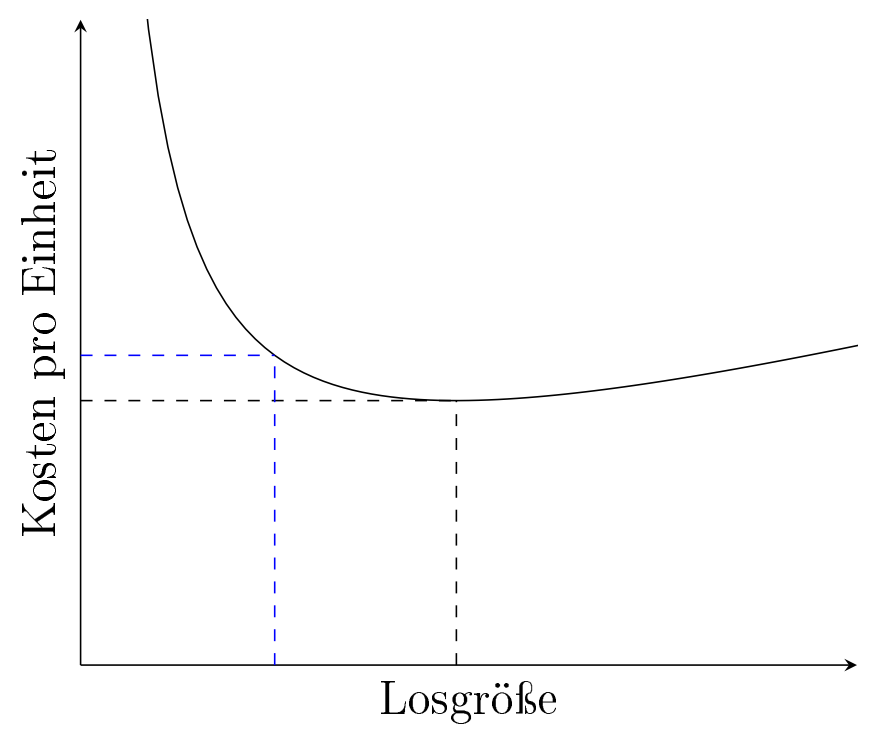
\includegraphics[width=.60\textwidth]{img/losgroessenverkleinerung.png}
\caption[Kosten bei Verkleinerung der Losgröße]{Kosten bei Verkleinerung der Losgröße\footnotemark}
\label{Losgroesse}
\end{figure}
\footnotetext{eigene Darstellung}

Letztlich muss aber auch daran gearbeitet werden, die Umrüstzeiten zu optimieren.
So ist es zum Beispiel Toyota gelungen, in seinem Hauptwerk die Zeit für Umrüstungen von 
2-3 Stunden in den 1940er Jahren auf nur 3 Minuten im Jahr 1971 zu reduzieren. \footnote{vgl. \cite{Ohno2013TPS} S.32f}

\subsection{Auswahl der Regelkreise}
Hat man die Kanban-fähigen Teile identifiziert, so müssen als nächstes die Regelkreise festgelegt werden, welche mit dem Kanban-System gesteuert werden sollen.
Dazu sollten zuerst von den betreffenden Abläufen Material- und Informationsflussdiagramme erstellt und die Prozessabläufe dargestellt werden.
Hierbei kann bereits versucht werden, Optimierungsmöglichkeiten zu realisieren \footnote{vgl. \cite{Geiger2011Kanban} S.35}. 
Schliesslich werden die am besten geeigneten Prozesse für die Kanban-Steuerung ausgewählt, 
inkl. Produzent und Verbraucher der Teile und ggf. der Zwischenlager.

\subsection{Ermittlung der Kanban-Größen}
Für die Kanban-Steuerung sind diese Kennzahlen relevant: Losgröße, Wiederbeschaffungszeit, 
Sicherheitsbestand, Maximalbestand, Kanban-Standardmenge und Kanban-Anzahl.\footnote{vgl. \cite{Geiger2011Kanban} S.36}\\

Wie bereits erwähnt sollte die \textbf{Losgröße} soweit wie möglich reduziert werden. Die positiven Effekte daraus sind  
höhere Flexibilität, geringere Lagerhaltungskosten, bessere Kundenorientierung, 
geringeres Abschreibungsrisiko, Vorteile beim Handling und Motivation der Mitarbeiter durch 
abwechslungsreichere Tätigkeit.\footnote{\cite{Geiger2011Kanban} S.36}\\

Für die \textbf{Wiederbeschaffungszeit} kann man die Erfahrungswerte mit den vorgelagerten Fertigungsstufen heranziehen.
Falls die Teile extern eingekauft werden, so muss mit dem Lieferanten eine realistische Wiederbeschaffungszeit vereinbart werden.\\

Der \textbf{Sicherheitsbestand} muss die Versorgung mit Teilen während der Wiederbeschaffungszeit ermöglichen.\\
\centerline{\textit{SB = DV * ( WBZ + SZ )}}
SB=Sicherheitsbestand\\
DV=Durchschnittsverbrauch pro Zeiteinheit\\
WBZ=Wiederbeschaffungszeit (in Zeiteinheiten)\\
SZ=Sicherheitszuschlag (in Zeiteinheiten)\\
Der Sicherheitszuschlag soll unvorhergesehene Bedarfsschwankungen oder Lieferprobleme
ausgleichen und sollte möglichst niedrig gewählt werden.\\

Die \textbf{Maximale Bestandsmenge} gibt an, wie viele Teile maximal im jeweiligen Kanban-Kreis vorhanden sein können.\footnote{vgl. \cite{Geiger2011Kanban} S.38}

\centerline{\textit{MB = WBZ * DV + BM + SB}}
 MB=Maximale Bestandsmenge\\
 WBZ=Wiederbeschaffungszeit (in Zeiteinheiten)\\
 DV=Durchschnittsverbrauch pro Zeiteinheit\\
 BM=Bestellmenge bzw. Losgröße\\
 SB=Sicherheitsbestand\\
Die Maximale Bestandsmenge sollte auch so weit wie möglich reduziert werden, da der Wert die Durchlaufzeit und das Umlaufvermögen beeinflußt.\\

Die \textbf{Kanban-Standardmenge} ist die Menge, die duch ein Kanban angefordert wird.
Sie sollte am besten einem vollen Behälter entsprechen und sich an der Losgröße orientieren.
Sollte die Losgröße grösser sein, z.B. weil bei einem Lieferanten immer eine bestimmte Mindestmenge angefordert werden muss, 
so werden die Kanban gesammelt, bis die Losgröße erreicht ist.\\

Die \textbf{Anzahl der Kanban} ergibt sich aus den anderen Größen:\footnote{vgl. \cite{Geiger2011Kanban} S.39}

\centerline{\textit{AK = (DV * WBZ * (1 + SF) ) / SM}}

 AK=Anzahl Kanban\\
 DV=Durchschnittsverbrauch pro Zeiteinheit\\
 WBZ=Wiederbeschaffungszeit (in Zeiteinheiten)\\
 SF = Sicherheitsfaktor\\
 SM = Standardmenge\\
Auch diese Kennzahl sollte möglichst klein gehalten werden. Sind zu viele Kanban-Karten im Umlauf so 
werden die Schwachstellen im Produktionssystem durch zu hohe Lagerbestände überdeckt.

Nach Einführung des Kanban-Systems sollten im Rahmen des \textit{kontinuierlichen Verbesserungsprozess} (KVP bzw. Kaizen) 
durch den Kanban-Verantwortlicher die Kanban-Größen regelmäßig geprüft und korrigiert werden. 

\subsection{Auswahl der Kanban-Hilfsmittel}
Die \textbf{Kanban-Karten} sind der eigentliche Namensgeber des Kanban-Systems und dienen der einfachen Informationsübertragung.
Jede Karte muss dazu mindestens diese Angaben enthalten: Verbraucher, Lieferant, Artikelbezeichnung, Artikelnummer, 
Angaben zum Behältnis und Mengenangaben (s. Abbildung \ref{Kanbankarte}). 
Zur erleichterten Datenerfassung kann auch ein Strich- oder QR-Code aufgedruckt sein.
Auch eine automatisierte und berührungslose Datenerfassung mittels Funketiketten (RFID) wird heute praktiziert.\footnote{vgl. \cite{Weber2014KE} S.100}
Sind weitere Angaben für einen sicheren und zuverlässigen Ablauf erforderlich, so sollten diese auch aufgenommen werden.
\footnote{vgl. \cite{Geiger2011Kanban} S.41}
Es gibt \textit{Produktions-Kanban}, die das Signal zur Produktion von Teilen geben, 
und Transport-Kanban welche das Signal zum Transport von Teilen geben.
Je nach den Gegebenheiten im Betrieb können diese auch kombiniert werden. Es gilt des Prinzip 'So einfach wie möglich.'
\footnote{vgl. \cite{Geiger2011Kanban} S.40}\\

Eine \textbf{Kanban-Tafel} hilft, die Übersichtlichkeit und Sicherheit des Systems zu gewährleisten. 
Hier werden die Karten der leeren Behälter gesammelt und in Spalten oder Zeilen angeordnet.  
Auf der Kanban-Tafel gibt es grüne, gelbe und rote Bereiche, so dass auf einen Blick erkennbar ist, wann neue Teile gefertigt werden müssen. (roter Bereich).
Im gelben Bereich kann der Verantwortliche selber entscheiden, ob er schon neue Teile produziert oder noch abwartet.\\

Die \textbf{Behälter} dienen dem Transport und der Lagerung der Teile, idealerweise kann für beides der gleiche 
Behälter verwendet werden, so dass die Teile nicht umgefüllt werden müssen. Behälter sollten 
zweckmäßig sein und orientieren sich an den Gegebenheiten vor Ort und den Eigenschaften der Teile, 
die Anzahl der Teile pro Behälter sollte der Losgröße entsprechen.
Für kleine C-Teile eignen sich kleine Plastik-Boxen, für größere Teile können Eurogitterboxen 
oder Transportwägen verwendet werden.\\
Behälter können auch gleichzeitig als Signal verwendet werden und somit die Kanban-Karten ersetzen: ein leerer 
Behälter ist ein Signal zur Produktion neuer Teile und muss von der Quelle unbedingt 
wieder in der vereinbarten Zeit mit neuen Teilen befüllt werden.\\
Auch Europaletten können als 'Behälter' im Sinne von Kanban verwendet werden, z.B. für grössere und schwere Teile.
Bei der Verwendung von Paletten können Stellflächen (des Zwischenlagers beim Verbraucher) als Signale dienen: 
ist nur noch eine Stellfläche mit einer Palette belegt, so muss nachgeliefert werden, sind alle Stellflächen belegt, 
darf nicht weiter produziert werden, dazwischen befindet sich der 'gelbe Bereich'.

\subsection{Erfassung von Daten}
Die Erfassung und Auswertung von betrieblichen Daten ist in der Regel unerlässlich.
Die dienen zur Kontrolle der Fertigung, Erstellung von Metriken und als Eingabedaten für das betriebliche EDV-System.
Als sinnvoll für die Datenerfassung haben sich Barcode-Lesegeräte und RFID-Systeme erwiesen. \footnote{vgl. \cite{Geiger2011Kanban} S.59}
Auf diese Weise können zusätzliche Papiere und Fehler durch Fehleingaben vermieden werden.
Die Lesegeräte können dann direkt mit den EDV-Systemen des Betriebes oder des Lieferanten verbunden werden.
Moderne ERP-Systeme wie z.B. von SAP unterstützen Kanban bereits direkt.\footnote{vgl. \cite{Weber2014KE} S.100}

\section{Kaizen: kontinuierliche Verbesserung}
Ein wichtiger Aspekt von JIT-Produktion mit Kanban ist, dass das ganze System stetig verbessert werden kann und soll.
Diesen Prinzip wird \emph{Kaizen} ({\CN 改善}) genannt, was so viel heisst wie Veränderung zum Besseren, 
heute auch bekannt unter dem Begriff \emph{kontinuierlicher Verbesserungsprozess} (KVP).
Jeder Mitarbeiter ist daher angehalten, permanent auf Optimierungspotential zu achten und Verbesserungsvorschläge zu machen.
Dies ist auch Ausdruck einer typisch japanischen Sichtweise: \emph{Der Einzelne ist Teil des Ganzen.}
Hat man eine Verbesserung erreicht, so wird diese zum neuen Standard gemacht und im gesamten Unternehmen eingeführt.

Ein Mittel für Verbesserung ist die Anzahl der Kanban-Karten.
Man beginnt daher bei Einführung von Kanban mit einer grösserer Anzahl von Kanban-Karten, und reduziert diese dann schrittweise.
So werden irgendwann unweigerlich Probleme in der JIT-Fertigung sichtbar, die nicht mehr mit hohen Lagerbeständen überdeckt werden können.

Jeder soll auch sofort Störungen und Fehler melden. 
Bei Toyoto geht das so weit, das jeder Arbeiter jederzeit das gesamte Band anhalten kann.
Denn je früher ein Fehler entdeckt und behoben wird, um so weniger kostet es.

Beim TPS  wird Wert darauf gelegt, der wirklichen Ursache eines Fehlers auf den Grund zu gehen.
Daher soll man 5 mal nach dem 'Warum' fragen, um das eigentliche Problem zu finden und zu beheben. \footnote{vgl. \cite{Toyota} }\\
Ein Fehler wird dabei nicht als etwas Schlechtes angesehen, sondern als eine Möglichkeit es besser zu machen - Fehler sollten immer zu Verbesserungen führen.

\section{Risiken von Just-in-Time}
Auch bei der JIT-Produktion kann es natürlich zu unvorhersehbaren Störung durch äußere Einflüsse kommen.
Durch Unwetter, Naturkatastrophen, Unfälle oder oder Streiks kann es zu verzögerter oder komplett ausfallenden Lieferungen durch externe Lieferanten kommen.
Auch interne Ereignisse wie z.B. Betriebsunfälle können die Fertigung erheblich beeinträchtigen.
Derartige Störungen müssen im Sinne von Kaizen ein entsprechend verbessertes Risiko-Management zur Folge haben.\\
Der Ausfall eines Lieferanten könnte z.B. zur Folge haben, dass künftig ein zweiter Lieferant für das 
gleiche Material eingebunden wird, mit der vertraglichen Vereinbarung, bei Bedarf die Lieferungen kurzfristig erhöhen zu können.\\
Sollte es durch einen großen Vulkanausbruch zu einem kompletten Ausfall der Frachtflüge kommen und 
wichtige Teile so nicht mehr geliefert werden können, dann könnte eine Folge des Risikomanagements sein, 
daß künfig bei wichtigen Teilen ein alternativer Transportweg via Strasse oder Schiene möglich ist.

Ein weitere Gefahr besteht darin, dass die JIT-Produktion nicht richtig umgesetzt wird, wobei auch schon Kleinigkeiten entscheidend sein können.
Grundsätzlich empfielt es sich daher vor allem in der Einführungsphase, den Rat von externen Experten einzuholen, 
welche bereits viel Erfahrung mit Kanban und JIT haben, und so die Fehler erkennen können.

\section{Fazit und Ausblick}
In der Arbeit wurde ein Überblick über die Just-in-Time-Produktion mit dem Kanban-System gegeben.
Es wurde gezeigt, wie und mit welcher Motivation diese Fertigungsmethode bei der japanischen Firma Toyota entwickelt wurde.
Toyota hat bewiesen, dass man mit diesen Methoden erfolgreich am Markt bestehen kann und hat sich so zu einem der größten Automobilhersteller weltweit entwickelt.
Das gesamte sog. Toyota-Produktionssystem umfasst aber noch viel mehr Aspekte, wie Autonomation (automatische Abschaltung bei Fehlern), 
Details des Qualitätsmanagements, standardisierte Arbeit, die '6 S', die 7 Verschwendungsarten oder die 3-Mu-Liste, um nur einige zu nennen. 
Diese sind jedoch nicht Gegenstand dieser Arbeit gewesen und können in weiteren Arbeiten untersucht und dargestellt werden. Des Weiteren könnte untersucht werden, 
welche Verbreitung Kanban, JIT- bzw. Lean-Production inzwischen gefunden haben und welche konkreten Verbesserungen dabei erreicht wurden.

